\cotefile{37}
\scanpage{47}

\diagram{\begin{tikzcd}[ampersand replacement=\&,column sep=large]
 E' \arrow[r,shift right=.55ex,"\varphi'"'] \&
 E'' \arrow[l,shift right=.55ex,"\varphi''"']
\end{tikzcd}
\quad
\begingroup
\setbox0=\hbox{$\left\{\begin{aligned}
\deleted{\lambda'\colon\operatorname{id}_{E'}\longrightarrow\unsure{\varphi'|\varphi}\varphi''}\\
\deleted{\lambda''\colon\operatorname{id}_{E''}\longrightarrow\varphi''\unsure{\varphi'|\varphi}}
\end{aligned}\right.$}
\dimen0=\dimexpr\ht0+\dp0\relax
\makebox[0pt][l]{\begin{tikzpicture}[overlay,x=\wd0,y=\dimen0]
\draw[thin] (.02,-.02)
 .. controls (.25,.70) and (.34,.54) .. (.24,-.34)
 .. controls (.55,.43) and (.70,.72) .. (.55,-.29)
 .. controls (.87,.31) and (.98,.78) .. (.86,-.14)
 .. controls (1.01,.11) and (1.03,.37) .. (.96,-.27)
 .. controls (.96,-.43) and (1.02,-.36) .. (1.05,-.30);
\end{tikzpicture}}%
\box0
\endgroup}

\diagram{\resizebox{\linewidth}{!}{\begin{tikzpicture}[x=.013cm,y=-.013cm,font=\footnotesize]
\node at (235,30) {\deleted{Esp fin}};
\node at (730,20) {\deleted{ord fin}};
\node at (242,190) {\deleted{\unsure{Espaces|Espace} \unsure{topologiques|top. quelconques|top. généraux} finis}};
\node at (850,165) {\deleted{ens préordonnés finis}};
\node at (280,308) {\deleted{espaces sobres finis}};
\node at (880,285) {\deleted{ens ordonnés finis}};
\node at (323,438) {\deleted{\unsure{ens. ordonné fini modulaire|ens. ordonnés finis modulaires|ens. ordonnés finis ou dual}}};
\draw[<->] (400,28) -- (625,28);
\draw[<->] (230,65) -- (235,137);
\node at (337,106) {\deleted{topologie opposée}};
\draw (756,50) .. controls (750,65) and (758,101) .. (760,120)
 .. controls (762,132) and (751,132) .. (750,124);
\draw (756,50) -- (765,55);
\node at (888,84) {\deleted{ordre opposé}};
\draw[<->] (527,165) -- (597,165);
\node at (593,126) {$\deleted{X\mapsto X\ \text{avec rel. spéc}}$};
\node[align=center] at (490,216) {\deleted{topologie}\\\deleted{des cribles}};
\node at (578,203) {$\deleted{\mathrel{\reflectbox{$\mapsto$}}X}$};
\draw[->] (227,235) .. controls (228,254) and (231,264) .. (235,270);
\draw[->] (808,210) .. controls (808,242) and (815,262) .. (823,265);
\draw[->] (615,294) -- (537,294);
\draw[<->] (239,340) -- (239,405);
\draw[thin] (226,-75) -- (60,352) -- (68,345);
\draw[thin] (390,-28) -- (191,466) -- (204,450);
\draw[thin] (547,25) -- (347,492) -- (357,484);
\draw[thin] (769,45) -- (590,435) -- (600,427);
\draw[thin] (952,96) -- (804,351) -- (810,347);
\draw[thin] (1036,175) .. controls (1029,207) and (987,272) .. (982,285);
\end{tikzpicture}}}

\diagram{\resizebox{\linewidth}{!}{\begin{tikzpicture}[x=.013cm,y=-.013cm,font=\footnotesize]
\node at (125,45) {$\widehat{\mathrm E}$sp fin};
\node at (546,32) {préord fin};
\node at (170,160) {$X=(\mathscr X,T)\in\widehat{\mathrm E}\text{sp fin \unsure{sob|sb}}$};
\node at (665,125) {$\text{ord fin}\ni(\mathscr X,\omega)=I$};
\node at (471,266) {$\text{Lat fin mod }\sigma$};
\node at (510,386) {Top fin spec};
\draw[<->] (240,50) -- (451,40);
\draw[->] (145,84) .. controls (149,101) and (162,113) .. (178,122);
\draw[->] (514,64) .. controls (522,91) and (527,100) .. (537,100);
\draw[<->] (323,152) -- (506,139);
\draw[<->] (235,194) -- (338,275);
\node at (351,188) {$X\to\operatorname{Ouv}(X)$};
\node at (359,211) {\deleted{\unsure{ens des ouverts|ens des ouverts.|ens. des ouverts}}};
\draw[<->] (594,154) -- (546,236);
\node at (645,198) {ens des cri};
\draw[->] (438,347) .. controls (424,332) and (424,304) .. (439,295);
\draw[line width=.6pt] (438,347) -- (445,352) -- (442,343);
\draw[->] (468,296) -- (480,365);
\node at (375,316) {$E\mapsto\operatorname{Ouv}(E)$};
\node at (560,316) {$\sigma\to\sigma^\sim$};
\draw[->,thin] (503,340) .. controls (539,350) and (592,336) .. (612,335);
\node at (674,338) {top can};
\draw[->] (187,194) .. controls (175,315) and (322,332) .. (388,367);
\node at (202,337) {$\operatorname{Top}(X,T)$};
\draw[->,thin] (293,427) .. controls (65,430) and (76,314) .. (102,234);
\node at (77,375) {$E\to\operatorname{Point}(E)$};
\draw[->] (764,157) .. controls (870,283) and (770,350) .. (681,391);
\node at (873,280) {$(X,\omega)^\wedge$};
\draw[->,thin] (733,398) .. controls (1094,370) and (1010,247) .. (860,164);
\node at (1088,302) {$\unsure{\underline{\underline E}|\underline E|E}\to\text{\uline{Point}}(E)$};
\node at (1080,47) {$\deleted{\unsure{y\leftarrow x|y\to x}}$};
\draw[line width=.9pt] (1097,11) .. controls (1092,24) and (1074,30) .. (1059,29);
\draw[line width=.9pt] (1059,29) -- (1069,35);
\draw[line width=1.2pt] (1097,11) -- (1088,4);
\draw[line width=.7pt] (1097,11) -- (1102,3);
\node at (953,115) {$x\longleftarrow y$};
\node at (897,159) {\unsure{spé.|spéc.}};
\node at (1000,159) {gén};
\end{tikzpicture}}}

\begin{flushright}
\begin{minipage}{.56\linewidth}
\deleted{\unsure{ensemble polye.|ensemble polyéd.|ensemble polyèdre}}\quad
schéma simplicial
\makebox[0pt][l]{\raisebox{1.7ex}{\inserted{fini}}}%
\makebox[0pt][l]{\tikz[overlay,x=1em,y=1ex]{\draw[thin] (-.05,1.0)
 .. controls (.05,1.5) and (.7,1.5) .. (1.4,1.5)
 .. controls (2.3,1.6) and (2.8,2.0) .. (2.65,2.9);}}%
\unsure{(}$=$ ens avec\\
\deleted{\unsure{anti|enti|ensemble}}\ \unsure{filtre des|filtres des|filtre de|filtres de} parties.

$\deleted{x\leq y\qquad x\longrightarrow y}$
\end{minipage}
\end{flushright}

\noindent\begin{minipage}[t]{.72\linewidth}
\vspace{0pt}
\diagram{\resizebox{\linewidth}{!}{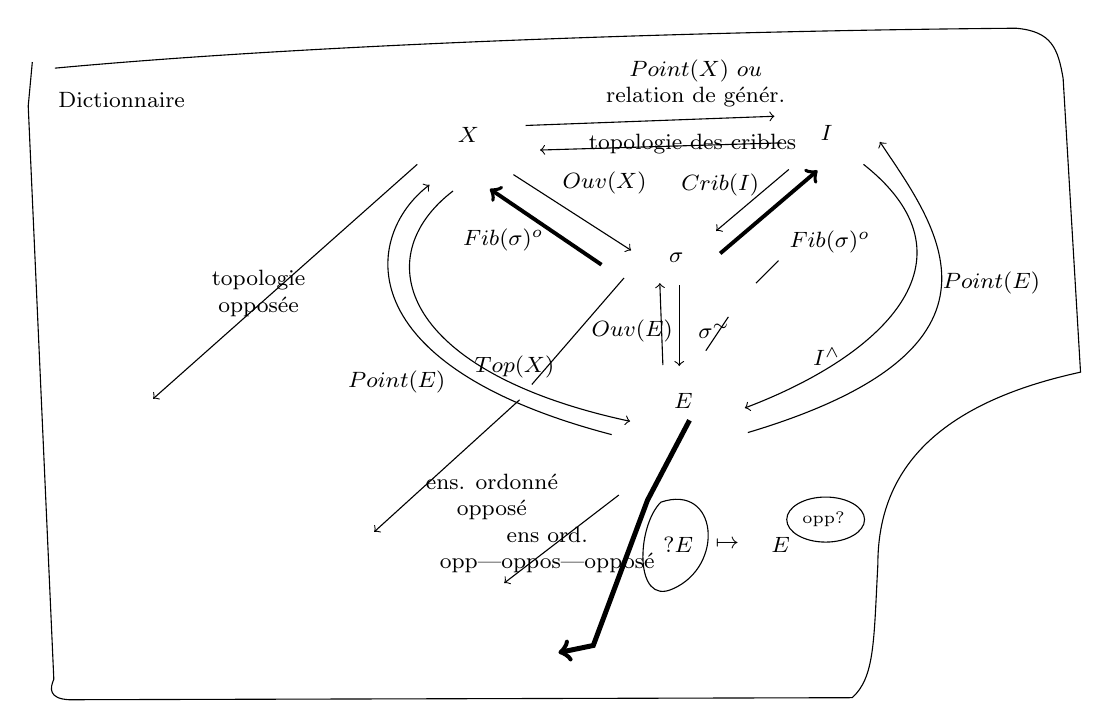
\begin{tikzpicture}[x=.013cm,y=-.013cm,font=\footnotesize]
\draw (26,45) .. controls (307,19) and (713,8) .. (965,6)
 .. controls (1000,9) and (1006,26) .. (1011,55)
 -- (1028,342)
 .. controls (876,375) and (830,447) .. (830,530)
 .. controls (826,605) and (827,640) .. (805,660)
 -- (40,662)
 .. controls (20,661) and (21,651) .. (25,642)
 -- (0,82) -- (4,39);
\node[anchor=west] at (20,76) {\uline{Dictionnaire}};
\node at (430,110) {$X$};
\node at (780,108) {$I$};
\node at (633,230) {$\sigma$};
\node at (640,370) {$E$};
\draw[->] (486,101) -- (729,92);
\draw[->] (736,118) -- (500,125);
\node[align=center] at (652,60) {$\text{\uline{Point}}(X)\ \text{ou}$\\relation de génér.};
\node at (649,119) {topologie des cribles};
\draw[->] (474,149) -- (589,223);
\draw[->,line width=1.4pt] (560,237) -- (451,163);
\node at (563,157) {$\operatorname{Ouv}(X)$};
\node at (464,213) {$\operatorname{Fib}(\sigma)^o$};
\draw[->] (743,144) -- (672,204);
\draw[->,line width=1.4pt] (676,226) -- (771,145);
\node at (676,159) {$\operatorname{Crib}(I)$};
\node at (783,215) {$\text{\uline{Fib}}(\sigma)^o$};
\draw[->] (620,335) -- (617,255);
\draw[->] (636,257) -- (636,336);
\node at (590,302) {$\operatorname{Ouv}(E)$};
\node at (670,302) {$\sigma^\sim$};
\draw[->] (415,165) .. controls (330,230) and (365,342) .. (588,390);
\draw[->] (570,403) .. controls (310,335) and (328,208) .. (392,159);
\node at (360,352) {$\operatorname{Point}(E)$};
\node at (475,337) {$\operatorname{Top}(X)$};
\draw[->] (816,139) .. controls (930,229) and (842,323) .. (700,377);
\draw[->] (703,401) .. controls (981,318) and (886,198) .. (832,117);
\node at (941,255) {$\text{\uline{Point}}(E)$};
\node at (780,327) {$I^\wedge$};
\draw[->] (380,139) -- (122,368);
\node[align=center] at (225,265) {topologie\\opposée};
\draw (582,250) -- (492,354);
\draw[->] (480,369) -- (338,498);
\node[align=center] at (453,464) {ens. ordonné\\opposé};
\draw (733,233) -- (711,255);
\draw (684,288) -- (662,321);
\draw[->] (577,462) -- (465,548);
\node[align=center] at (507,516) {ens ord.\\\unsure{opp|oppos|opposé}};
\draw[->,line width=1.8pt] (646,389) -- (605,467) -- (552,609) -- (518,616);
\node[inner sep=0pt] at (635,511) {$?E$};
\node[inner sep=0pt] at (683,510) {$\mapsto$};
\node[inner sep=0pt] at (735,511) {$E$};
\node[inner sep=0pt] at (777,486) {$\scriptstyle\mathrm{opp}?$};
\draw (618,469) .. controls (674,450) and (681,532) .. (629,554)
 .. controls (592,570) and (594,493) .. (618,469);
\draw (779,486) ellipse (38 and 22);
\end{tikzpicture}}}
\end{minipage}\hfill
\begin{minipage}[t]{.25\linewidth}
\vspace*{4.1cm}
\small
\[
I^\wedge\qquad I^\vee
\]
\noindent\makebox[0pt][r]{%
\makebox[0pt][l]{\tikz[overlay,x=1em,y=1ex]{
\draw[thin] (.2,.2) .. controls (.6,2.0) and (1.2,2.2) .. (1.35,1.7)
 .. controls (1.1,.9) and (.6,.3) .. (.2,.2);
\draw[thin] (1.2,.2) -- (2.1,1.9) -- (2.8,.5)
 .. controls (2.3,.0) and (1.6,.0) .. (1.2,.2);}}%
$\deleted{\unsure{X\to Y|X\leftrightarrow Y}}$\quad}%
\begingroup
\setbox0=\hbox{$C^\wedge\ \text{et}\ C^\vee={C^o}^\wedge$}%
\dimen0=\dimexpr\ht0+\dp0\relax
\makebox[0pt][l]{\begin{tikzpicture}[overlay,x=\wd0,y=\dimen0]
\draw[thin] (-.05,.25) .. controls (-.07,.67) and (-.04,.87) .. (.02,.83)
 -- (1.05,1.00) -- (1.08,-.12) -- (.00,-.28)
 .. controls (-.07,-.31) and (-.06,-.15) .. (-.05,.18);
\draw[line width=.7pt] (1.05,1.00) -- (1.06,-.04);
\end{tikzpicture}}%
\box0
\endgroup

\bigskip
\noindent\makebox[0pt][l]{\tikz[overlay,x=1em,y=1ex]{
\draw[thin] (8.2,1.4) .. controls (8.9,-.7) and (7.0,-1.6) .. (3.6,-1.6)
 .. controls (.1,-1.7) and (-1.4,-.8) .. (-1.2,.6)
 .. controls (-1.0,2.4) and (1.2,2.5) .. (4.0,2.1)
 .. controls (6.0,1.8) and (8.2,1.9) .. (8.2,1.65);}}%
to\uline{pos opposé} ?
\end{minipage}

% archive sheet number: 46

